\documentclass[a4paper]{article}
\usepackage[utf8x]{inputenc}
\usepackage[lastexercise]{exercise}
\usepackage{color}
\usepackage[absolute]{textpos} 
\usepackage{verbatim}
\usepackage{tikz}
\usetikzlibrary{calc}
\usetikzlibrary{positioning}
\usetikzlibrary{shapes.misc}
\usetikzlibrary{arrows}

\renewcommand\ExerciseName{Exercice}
\renewcommand{\AnswerHeader}{\medskip\centerline{\textbf{Solution de
                        l'\ExerciseName  \ExerciseHeaderNB}\smallskip}}
\newenvironment{CAnswer}{\color{red}\begin{Answer}}
                        {\end{Answer}}

\title{Prolog - TP2\\Récursion, Listes}
\date{}

\begin{document}
\maketitle
\begin{textblock*}{4cm}(10mm,10mm)
\begin{Large}ESIAL 3A IL LE\end{Large}
\end{textblock*}
\begin{textblock*}{3cm}(160mm,10mm)

\includegraphics[width=\textwidth]{../../ESIAL.pdf}
\end{textblock*}

\begin{Exercise}[title={Quelques tests}]
Sans lancer les requêtes, devinez quel est le résultat des requêtes suivantes :
\Question \verb$?­ [] = _.$
\Question \verb$?­ [_] = [].$
\Question \verb$?­ [_ | _] = [_].$
\Question \verb$?­ [_ | [_]] = [_].$\\
Testez ensuite vos résultats avec Prolog.
\end{Exercise}
\begin{CAnswer}
\begin{verbatim}
?­ [] = _.
yes
?­ [_] = [].
no
?­ [_ | _] = [_].
yes
?­ [_ | [_]] = [_].
no
\end{verbatim}
\end{CAnswer}

\begin{Exercise}[title={Poupées russes}]
On souhaite pouvoir représenter un jeu de poupées russes. Représentez la
situation suivante :
\begin{center}
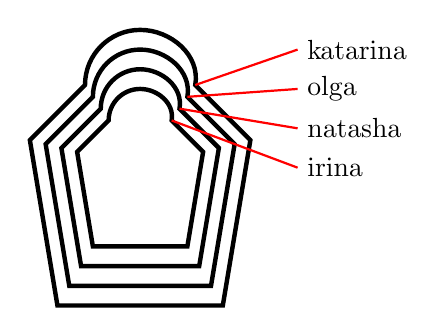
\begin{tikzpicture}[nodes={minimum size=1.5em}]
 \foreach \x in {4,5,6,7} {
 \draw[scale=\x*.05,ultra thick] (3,-5) -- (4,1) -- (2,3) coordinate (p\x)
       to [out=80,in=0] (0,5) 
       to [out=180,in=90] (-2,3) -- (-4,1) -- (-3,-5) -- cycle;
 } 
 \draw (2, .0) node [anchor=west] {irina} [red,thick] -- (p4);
 \draw (2, .5) node [anchor=west] {natasha} [red,thick] -- (p5);
 \draw (2, 1.) node [anchor=west] {olga} [red,thick] -- (p6);
 \draw (2, 1.5) node [anchor=west] {katarina} [red,thick] -- (p7);
\end{tikzpicture} 
\end{center}
Ecrivez le prédicat \verb$dans/2$, vrai si une poupée est dans une autre peu
importe son niveau d'imbrication. Vous pourrez vous appuyer sur un prédicat
\verb$directementDans/2$, vrai si une poupée est directement dans une autre.
\end{Exercise}
\begin{CAnswer}
\verbatiminput{poupee_russes.pro}
\end{CAnswer}

\begin{Exercise}[title={Dernier}]
Ecrivez le prédicat \verb$dernier/2$, vrai lorsque le second argument est le
dernier élément de la liste donnée en premier argument. Par exemple :
\begin{verbatim}
?­ dernier([a,b,c], c).
yes
\end{verbatim}
\end{Exercise}
\begin{CAnswer}
\verbatiminput{dernier.pro}
\end{CAnswer}

\begin{Exercise}[title={Inversion}]
\Question Ecrivez le prédicat \verb$inverse/2$, vrai lorsque la seconde liste
est une inversion de la première liste. Par exemple :
\begin{verbatim}
?­ inverse([a,b,c,d], [d,c,b,a]).
yes
\end{verbatim}
Vous pouvez éventuellement vous appuyer sur le prédicat \verb$append/3$.
\Question Ecrivez ensuite le prédicat \verb$palindrome/1$, qui teste si une
liste est un palindrome\footnote{un palindrome est un mot qui se lit de la
même façon de droite à gauche que de gauche à droite}. Par exemple :
\begin{verbatim}
?­ palindrome([n,o,n]).
yes
?­ palindrome([o,u,i]).
no
\end{verbatim}
Testez \verb$palindrome([o,u|Y]).$.
\Question Vous pouvez réécrire le prédicat \verb$dernier/2$ très facilement
avec le prédicat \verb$inverse/2$. Comment faire ?
\end{Exercise}
\begin{CAnswer}
\verbatiminput{inversion.pro}
\end{CAnswer}

\begin{Exercise}[title={Plus longue}]
\Question Ecrivez le prédicat \verb$pluslongue/2$, vrai si la première liste
est strictement plus longue que la seconde. Par exemple:
\begin{verbatim}
?­ pluslongue([a,b,c], [d,e]).
yes
\end{verbatim}
\Question Ecrivez le prédicat \verb$lapluslongue/2$, tel que le premier
argument soit une liste de listes, et le second argument la liste la plus
longue strictement appartenant à cette liste. Par exemple :
\begin{verbatim}
?­ lapluslongue([[a,b], [c,d,e], []], X).
X = [c,d,e]
yes
\end{verbatim}
\end{Exercise}
\begin{CAnswer}
\verbatiminput{plus_longue.pro}
\end{CAnswer}

\begin{Exercise}[title={Voyage}]
On cherche à déterminer les trajets qui existent entre deux villes :
\begin{center}
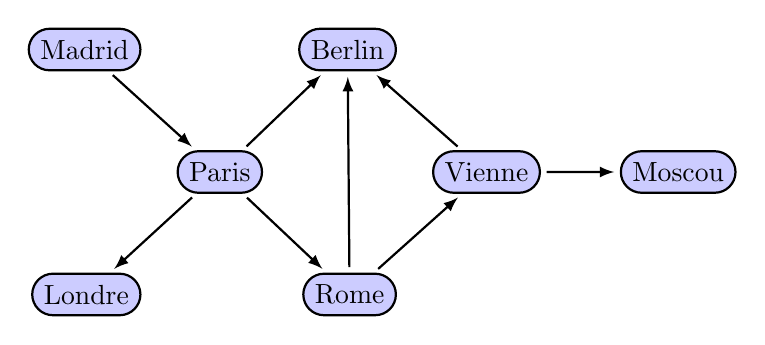
\begin{tikzpicture}[nodes={draw, rounded rectangle, fill=blue!20, 
			   minimum size=1.5em},
		    every path/.style={draw, -latex,shorten >=2pt, shorten <=2pt},
                    thick]
 \node (moscou) {Moscou};
 \node [left=of moscou] (vienne) {Vienne};
 \node [above left=of vienne] (berlin) {Berlin};
 \node [below left=of vienne] (rome) {Rome};
 \node [below left=of berlin] (paris) {Paris};
 \node [above left=of paris] (madrid) {Madrid};
 \node [below left=of paris] (londre) {Londre};

 \path (madrid) edge (paris)
       (paris)  edge (berlin) 
		edge (rome) 
                edge (londre)
       (rome)   edge (berlin)
		edge (vienne)
       (vienne) edge (berlin)
		edge (moscou);
\end{tikzpicture} 
\end{center}
\Question Ecrivez un prédicat \verb$voyage/3$, dont le premier argument est une
ville de départ, le second argument une ville de destination, et le troisième
argument la liste des villes qu'il faut traverser pour se rendre de la ville de
départ à la ville de destination. On doit avoir :
\begin{verbatim}
?­ voyage(madrid, vienne, [paris, rome, vienne]).
yes
\end{verbatim}
Testez votre prédicat avec des variables, par exemple pour obtenir la liste des
trajets possibles entre deux villes, ou l'ensemble des villes accessibles étant
donné une ville de départ et un trajet.

\Question Appuyez vous sur ce qui a été fait dans l'exercice précédent pour
écrire le prédicat \verb$lepluscourtvoyage/3$, qui renvoie le voyage le plus
court entre deux villes. Vous pourrez utiliser le prédicat \verb$findall/3$ qui
permet de rassembler dans une liste tous les résultats d'une requête. Par
exemple, si on a :
\begin{verbatim}
p(a).
p(b).
p(c).
?­findall(X, p(X), L).
L = [a,b,c].
\end{verbatim}
Le premier argument désigne la variable correspondant aux éléments de la liste
résultat, le second argument la condition que doit satisfaire la variable et le
troisième argument désigne la liste résultat.
\end{Exercise}
\begin{CAnswer}
\verbatiminput{voyage.pro}
\end{CAnswer}

\end{document}
